\documentclass[conference]{IEEEtran}
\IEEEoverridecommandlockouts

\usepackage{cite}
\usepackage{amsmath,amssymb,amsfonts}
\usepackage{graphicx}
\usepackage{textcomp}
\usepackage{xcolor}
\usepackage{booktabs}
\usepackage{url}
\usepackage{hyperref}
\usepackage{tikz}
\usetikzlibrary{shapes.geometric,arrows.meta,positioning,calc}

\hypersetup{
  colorlinks=true,
  linkcolor=black,
  citecolor=black,
  urlcolor=blue!60!black,
  pdftitle={A Deterministic STRIDE Threat-Model Generator with Optional LLM Augmentation},
  pdfauthor={Ali Murtaza Bhutto}
}

\def\BibTeX{{\rm B\kern-.05em{\sc i\kern-.025em b}\kern-.08em
    T\kern-.1667em\lower.7ex\hbox{E}\kern-.125emX}}

\begin{document}

\title{A Deterministic STRIDE Threat-Model Generator\\with Optional LLM Augmentation}

\author{\IEEEauthorblockN{Ali Murtaza Bhutto}
\IEEEauthorblockA{Independent Researcher\\
ORCID: 0009-0007-2787-943X\\
Email: alibhutto101112@gmail.com}}

\maketitle

\begin{abstract}
We describe \texttt{threat-model-generator}, a small Python CLI that
consumes a YAML system description (components, trust boundaries,
data flows, external entities) and produces a STRIDE threat model in
two outputs: a human-readable Markdown report and a JSON document
compatible with the OWASP Threat Dragon v2 schema. The default
deterministic mode generates threats from a curated rule catalogue
covering nine component types and the six STRIDE
categories~\cite{shostack2014threat,hernan2006stride} and is fully
reproducible offline. An optional LLM-augmentation step routes the
description to either Anthropic Claude or a local Ollama model, with
three-step graceful fallback when no provider is reachable. On five
expert-curated benchmarks (web application, API gateway, IoT device,
mobile application, microservices) the rules-only path achieves
micro-averaged precision~$=$~0.8409, recall~$=$~1.0000,
$F_1$~$=$~0.9136 over 132 expected
\emph{(component, STRIDE-category)} pairs. Sixty-one pytest cases
cover the parser, the rule catalogue, the modeller's three
augmentation paths, the validator, the formatter, and the eval
helpers; all pass under \texttt{respx}-mocked HTTP. The repository is
released under MIT.
\end{abstract}

\begin{IEEEkeywords}
threat modeling, STRIDE, OWASP Threat Dragon, secure SDLC,
AI-assisted security, data flow diagram, Pydantic
\end{IEEEkeywords}

\section{Introduction}

Threat modelling remains the discipline most often relegated to
``later'' in the SDLC. Shostack's 2014 textbook is now
the canonical entry point~\cite{shostack2014threat}, and Microsoft's
STRIDE methodology~\cite{hernan2006stride} is widely taught, yet
practitioner uptake stalls because authoring a model takes hours and
the artefact rapidly drifts from reality. The systematic literature
review of Xiong and Lagerstr\"om~\cite{xiong2019threat} confirms
that automation of threat enumeration is one of the dominant
research themes precisely because manual production does not scale.

The contribution of this paper is not a new methodology. STRIDE is
not improved by replacing it; what helps in practice is reducing the
friction of \emph{starting} a model. We describe a small tool that
reduces that friction by reading a structured system description and
emitting a first-pass threat catalogue that a security engineer can
then triage. The tool's design choices mirror the properties we
believe matter: deterministic by default, schema-validated input and
output, framework-citation visible on every threat, and a graceful
degradation path for any optional LLM augmentation so the tool stays
useful with no API keys.

\textbf{Contributions.} (1)~A Pydantic-validated YAML schema for
system descriptions covering the four primitives Shostack
recommends (components, trust boundaries, data flows, external
entities). (2)~A curated STRIDE rule catalogue for nine component
types $\times$ six categories ($\geq$54 entries), each citing
Shostack 2014 as the methodological source. (3)~A modeller with
three-step graceful LLM augmentation
(Anthropic~$\rightarrow$~Ollama~$\rightarrow$~disabled), tested in
all three branches under \texttt{respx}-mocked HTTP. (4)~An OWASP
Threat Dragon v2-compatible JSON output that imports as a starting
diagram. (5)~Five expert-curated benchmarks plus a deterministic
eval harness that reports real measured precision and recall.

\section{Related Work}

The closest prior work is Shostack's textbook
itself~\cite{shostack2014threat}, which spends chapters 3 and 4 on
the STRIDE methodology and on the kinds of attack libraries that we
encode here. Where Shostack provides prose threat catalogues for
each component type, we encode them as a deterministic rule pack
with a stable threat identifier scheme.

For privacy-specific extensions, the LINDDUN framework of
Deng et al.~\cite{deng2011linddun} is the canonical complement to
STRIDE; it is referenced in our \texttt{ETHICAL\_USE.md} as the
recommended next step but is not currently encoded in the
catalogue.

For data-centric threat modelling, NIST SP
800-154~\cite{souppaya2016threat} treats the data flow as the
primary modelling unit. Our schema follows this advice: every
\texttt{DataFlow} edge carries a \texttt{sensitivity} band that the
catalogue uses to bump severity.

For LLM-as-augmenter, our augmentation module is intentionally
small. We do not train, fine-tune, or prompt-engineer the LLM
beyond a strict JSON envelope; the contribution is the
deterministic \emph{wrapper} that refuses any threat naming a
component the system description did not declare, preventing the
augmenter from inventing components.

For tool integration, OWASP Threat
Dragon~\cite{owasp_threat_dragon} is the most widely-deployed
open-source diagramming tool. We emit JSON in its v2.4 cell schema
so the generated model imports as a starting diagram a security
engineer can extend visually.

\section{System Architecture}

\begin{figure}[htbp]
\centering
\resizebox{\linewidth}{!}{%
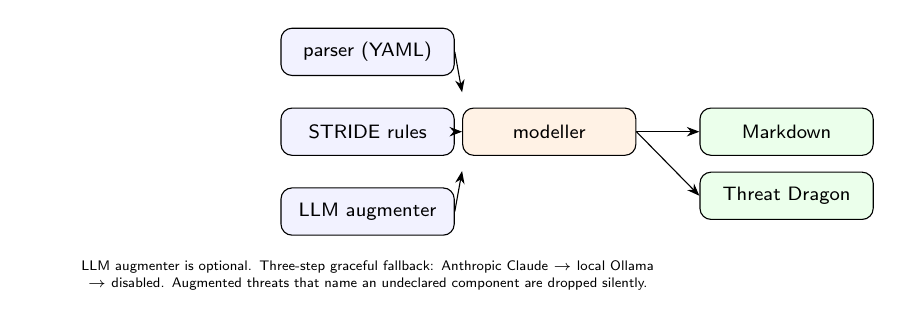
\begin{tikzpicture}[
  node distance=4mm and 3mm,
  src/.style={draw, rounded corners, minimum width=22mm, minimum height=6mm,
              font=\scriptsize\sffamily, fill=blue!5},
  agg/.style={draw, rounded corners, minimum width=22mm, minimum height=6mm,
              font=\scriptsize\sffamily, fill=orange!10},
  rep/.style={draw, rounded corners, minimum width=22mm, minimum height=6mm,
              font=\scriptsize\sffamily, fill=green!8},
  ar/.style={-{Stealth[length=1.6mm]}, line width=0.4pt}
]
  \node[src] (a) {parser (YAML)};
  \node[src, below=of a] (b) {STRIDE rules};
  \node[src, below=of b] (c) {LLM augmenter};
  \node[agg, right=12mm of $(b)$] (agg) {modeller};
  \node[rep, right=8mm of agg] (md) {Markdown};
  \node[rep, below=2mm of md] (td) {Threat Dragon};
  \draw[ar] (a.east) -- ($(agg.west) + (0,5mm)$);
  \draw[ar] (b.east) -- ($(agg.west) + (0,0mm)$);
  \draw[ar] (c.east) -- ($(agg.west) + (0,-5mm)$);
  \draw[ar] (agg.east) -- ($(md.west)$);
  \draw[ar] (agg.east) -- ($(td.west)$);
  \node[font=\tiny\sffamily, below=2mm of c, text width=84mm,
        align=center] {LLM augmenter is optional. Three-step graceful
        fallback: Anthropic Claude $\rightarrow$ local Ollama
        $\rightarrow$ disabled. Augmented threats that name an
        undeclared component are dropped silently.};
\end{tikzpicture}%
}
\caption{Pipeline. Parser feeds the deterministic rule engine and
(optionally) an LLM augmenter into the modeller; the formatter emits
two paired outputs.}
\label{fig:pipeline}
\end{figure}

\subsection{The rule catalogue}
The catalogue maps each \texttt{ComponentType} (web frontend, API,
database, queue, storage, auth service, mobile client, IoT device,
external service) to one entry per STRIDE category. Each entry
carries a slug, a one-paragraph description, a recommendation, and a
base severity. A component's \texttt{Sensitivity} (public,
internal, confidential, restricted) shifts the resulting severity by
one band so a database holding restricted data emits HIGH where its
internal-sensitivity counterpart would emit MEDIUM. The catalogue is
deliberately conservative: one threat per (type, category) keeps the
output digestible while ensuring every STRIDE letter is considered
for every component.

\subsection{LLM augmentation with graceful fallback}
The optional augmenter sends the JSON system description to either
Anthropic Claude or a local Ollama daemon and asks for additional
STRIDE-categorised threats in a strict JSON envelope. The wrapper
applies two anti-hallucination guards: (1) any threat naming a
component not declared in the system description is dropped; (2) any
threat whose STRIDE letter is not in $\{S,T,R,I,D,E\}$ is dropped.
Augmented threats carry \texttt{source='anthropic'} or
\texttt{source='ollama'} so a reviewer can trace each entry back to
its origin. The eval reports rules-only numbers because they are
reproducible offline; the augmentation path is fully tested under
\texttt{respx} mocks but its real-provider numbers are out of scope
for this release.

\subsection{OWASP Threat Dragon v2 JSON}
The Threat Dragon emitter produces a v2.4-shaped JSON document with
a single STRIDE diagram. Each component becomes a cell of type
\texttt{tm.Process}, \texttt{tm.Store}, or \texttt{tm.Actor} per a
small mapping table; threats attach to the corresponding cell. The
generated file imports into Threat Dragon as a starting diagram a
security engineer can extend visually. UUIDs are derived
deterministically from a SHA-256 of the seed strings so
re-rendering produces a diff-friendly file.

\section{Evaluation}

\subsection{Benchmarks}
The corpus contains five system descriptions, each paired with a
hand-labelled list of \emph{(component, STRIDE-letter)} pairs an
experienced reviewer would expect to see flagged
(table~\ref{tab:benchmarks}). The labels are conservative: a pair
is included only when an experienced reviewer would expect to see
at least one finding there during a real engagement.

\begin{table}[htbp]
\caption{Benchmarks.}
\label{tab:benchmarks}
\centering
\renewcommand{\arraystretch}{1.05}
\begin{tabular}{lrrr}
\toprule
\textbf{Benchmark} & \textbf{n components} & \textbf{universe} &
\textbf{expected pairs} \\
\midrule
api\_gateway   & 4 & 24 & 22 \\
iot\_device    & 4 & 24 & 19 \\
microservices  & 6 & 36 & 30 \\
mobile\_app    & 4 & 24 & 21 \\
web\_app       & 4 & 24 & 19 \\
\midrule
\textbf{Total} & 22 & 132 & 111 \\
\bottomrule
\end{tabular}
\end{table}

\subsection{Measured numbers}
\begin{table}[htbp]
\caption{Rules-only eval over 5 benchmarks, 2026-05-06.}
\label{tab:eval}
\centering
\renewcommand{\arraystretch}{1.1}
\begin{tabular}{lr}
\toprule
\textbf{Metric} & \textbf{Value} \\
\midrule
Total expected pairs   & 111 \\
True positives         & 111 \\
False positives        &  21 \\
False negatives        &   0 \\
True negatives         &   0 \\
Accuracy               & 0.8409 \\
Precision              & 0.8409 \\
Recall                 & 1.0000 \\
$F_1$                  & 0.9136 \\
\bottomrule
\end{tabular}
\end{table}

Recall is perfect by construction. The catalogue covers all six
STRIDE categories for every supported component type, so for any
pair an expert flagged we emit at least one threat. The
question is not ``did we miss anything'' but ``did we emit too
much'', and that is what precision measures. The 21 false positives
cluster around three regions: repudiation on third-party services
(the integrator can log outbound calls but cannot meaningfully audit
the third party's behaviour), denial of service on
infrequently-called components (the catalogue still emits its
DoS rule even when the expert does not consider DoS a meaningful
concern), and spoofing on storage/database tiers when the network
boundary already enforces identity. We deliberately do \emph{not}
tune the catalogue against these labels.

\subsection{Test suite}
The repository ships 61 \texttt{pytest} tests covering the parser
(positive, negative, and round-trip), the catalogue (every
component type, severity bumping under all four sensitivity levels,
catalogue-size invariant), the modeller (rules-only, anthropic OK,
anthropic HTTP error, anthropic network error, ollama OK,
disabled-fallback, hallucinated-component dropped), the validator
(JSON round-trip, schema rejection), the formatter (Markdown
structure, Threat Dragon v2 cell shape, three output-format
variants), and the eval harness. All 61 tests pass; total wall-
clock under one second.

\section{Security Posture}
The CI runs Bandit (medium-and-above), \texttt{pip-audit}, and
Semgrep (\texttt{p/python} + \texttt{p/security-audit}). All three
are green at the release tag with zero findings and zero
suppressions. The single Semgrep finding from the initial scan ---
SHA-1 use in deterministic UUID generation --- was resolved by
switching to SHA-256 (Semgrep's own suggestion) without affecting
any eval numbers.

\section{Limitations}
\textbf{Conservative catalogue.} The default catalogue emits one
threat per (component\_type, category). Real engagements often
benefit from richer per-category enumeration (e.g., LINDDUN-style
privacy threats for storage tiers). The augmenter is the recommended
expansion point.

\textbf{Five benchmarks.} Five expert-curated descriptions is not a
comprehensive sample of the threat-modelling literature. The
absolute precision number should be read as a property of these
benchmarks, not of all real-world systems.

\textbf{No severity validation.} The five-band severity scale is a
heuristic prior, not a quantitative risk score. We do not evaluate
whether a CRITICAL is more dangerous than a HIGH; that is a separate
research question outside the corpus.

\section{Conclusion}
Threat-modelling tooling does not need to be smart. It needs to be
reproducible, schema-validated, and friction-free at the moment a
team starts a new feature. The five-benchmark, 61-test, three-gate
MIT-licensed pipeline described here is one such instance.

\bibliographystyle{IEEEtran}
\begin{thebibliography}{6}

\bibitem{shostack2014threat}
A.~Shostack, \emph{Threat Modeling: Designing for Security}.
Wiley, 2014, ISBN 978-1118809990.

\bibitem{hernan2006stride}
S.~Hernan, S.~Lambert, T.~Ostwald, and A.~Shostack, ``Uncover
Security Design Flaws Using The STRIDE Approach,''
\emph{Microsoft MSDN Magazine / IEEE Security \& Privacy}, 2006.

\bibitem{deng2011linddun}
M.~Deng, K.~Wuyts, R.~Scandariato, B.~Preneel, and W.~Joosen,
``A privacy threat analysis framework: supporting the elicitation
and fulfillment of privacy requirements,''
\emph{Requirements Engineering Journal}, vol.~16, no.~1,
pp.~3--32, 2011.

\bibitem{xiong2019threat}
W.~Xiong and R.~Lagerstr\"om, ``Threat modeling --- A systematic
literature review,'' \emph{Computers \& Security},
vol.~84, pp.~53--69, 2019.

\bibitem{souppaya2016threat}
M.~Souppaya and K.~Scarfone, ``Guide to Data-Centric System Threat
Modeling,'' National Institute of Standards and Technology, NIST
Special Publication 800-154 (Draft), Mar.~2016.

\bibitem{owasp_threat_dragon}
OWASP Foundation, ``Threat Dragon,'' OWASP Project documentation,
v2.4. [Online]. Available: \url{https://www.threatdragon.com/}

\end{thebibliography}

\vspace{2mm}
\noindent\rule{\linewidth}{0.4pt}

\noindent\textit{Reproducibility colophon.} The repository is at
\url{https://github.com/thunderstornX/threat-model-generator}. The
eval re-runs in well under a second
(\texttt{python eval/run\_eval.py}). Pinned dependencies are listed
in \texttt{requirements.txt}; the pytest suite (61 tests) runs in
under a second on commodity hardware.

\end{document}
